%% This is file `DEMO-TUDaPub.tex' version 2.09 (2020/03/13),
%% it is part of
%% TUDa-CI -- Corporate Design for TU Darmstadt
%% ----------------------------------------------------------------------------
%%
%%  Copyright (C) 2018--2020 by Marei Peischl <marei@peitex.de>
%%
%% ============================================================================
%% This work may be distributed and/or modified under the
%% conditions of the LaTeX Project Public License, either version 1.3c
%% of this license or (at your option) any later version.
%% The latest version of this license is in
%% http://www.latex-project.org/lppl.txt
%% and version 1.3c or later is part of all distributions of LaTeX
%% version 2008/05/04 or later.
%%
%% This work has the LPPL maintenance status `maintained'.
%%
%% The Current Maintainers of this work are
%%   Marei Peischl <tuda-ci@peitex.de>
%%   Markus Lazanowski <latex@ce.tu-darmstadt.de>
%%
%% The development respository can be found at
%% https://github.com/tudace/tuda_latex_templates
%% Please use the issue tracker for feedback!
%%
%% ============================================================================
%%
% !TeX program = lualatex
%%

\documentclass[
	ngerman,
	accentcolor=1c,% Farbe für Hervorhebungen auf Basis der Deklarationen in den Corporate Design Richtlinien
%	logofile=example-image, %Falls die Logo Dateien nicht vorliegen
	]{tudapub}

\usepackage[english, main=ngerman]{babel}
\usepackage[babel]{csquotes}

\usepackage{biblatex}
\bibliography{DEMO-TUDaBibliography}

%Formatierungen für Beispiele in diesem Dokument. Im Allgemeinen nicht notwendig!
\let\file\texttt
\let\code\texttt
\let\pck\textsf
\let\cls\textsf

\usepackage{hologo}


\usepackage{floatrow}
%\usepackage{subfig}
\newfloatcommand{capbtabbox}{table}[][\FBwidth+5cm]
\usepackage{blindtext}
\usepackage{colortbl}
\usepackage{ifthen}

%\usepackage[demo]{graphicx}
\usepackage{caption}
\usepackage[skip=0cm,list=true,labelfont=it]{subcaption}


\newcommand{\unit}[1]{{\rm\,#1}}

\newboolean{sensorsDetailed}
\setboolean{sensorsDetailed}{true}

\begin{document}

%Zusätzliche Metadaten für PDF/A. In diesem Fall notwendig, weil Titel ein Makro enthält.
\Metadata{
	author=NeXT,
	title=Space Workshop Rating,
	%subject=Basisdokumentation und Template zur Nutzung der tudapub-Dokumentenkasse,
	%date=2019-04-29,
	%keywords=TU Darmstadt \sep Corporate Design \sep LaTeX
}




\title{Space Workshop\newline Bewertungsbogen}
\subtitle{NeXT Generation on Campus}
%\author{Marei Peischl\thanks{pei\TeX{} \TeX{}nical Solutions}\and der \TeX-Löwe}
\date{}
\titleimage{
%	%Folgende Box kann selbstverständlich durch ein mit \includegraphics geladenes Bild ersetzt werden.
\bigskip
\bigskip
\bigskip
\bigskip
\bigskip
\bigskip
\bigskip
\bigskip
\bigskip
\bigskip
\bigskip
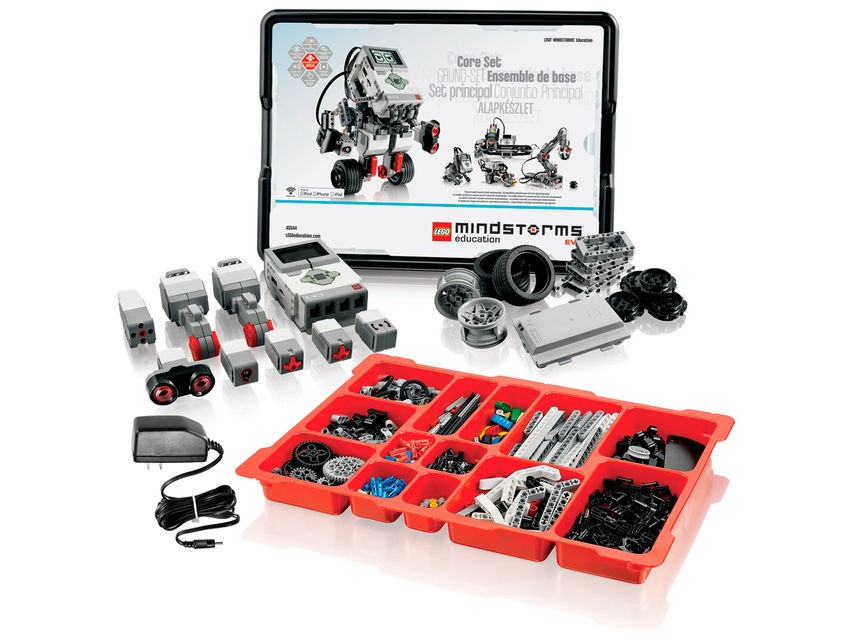
\includegraphics[width=\textwidth]{../control/images/title.jpg}
	%\color{black!30}\rule{\width}{\height}
}


%Varianten der Infoboxen
\addTitleBox{\includegraphics[width=\linewidth]{../control/images/ist_logo.pdf}}
%\addTitleBoxLogo{example-image}
%\addTitleBoxLogo*{\includegraphics[width=.3\linewidth]{example-image}}



\maketitle


\newpage

%\end{figure}
\bigskip
In diesem Wertungsbogen gibt es genauere Informationen, wie die Punkte im Wettkampf verteilt werden und worauf ihr vielleicht besonders achten solltet.
Die Teams treten nacheinander an und haben drei Versuche pro Station.
Vor dem Start muss einmal die bearbeitete Aufgabe genannt werden und ob Sensoren eingesetzt wurden.
Zu Beginn der Aufgabe muss der Roboter an einer der markierten Startpositionen stehen. F"ur die Bearbeitung der Aufgabe muss die Station komplett verlassen werden.
Wenn die Aufgabe nicht komplett gel"ost werden konnte, gibt es Teilpunkte. Pro Aufgabe gibt es mindestens 0 Punkte.\\
Wichtiger als die genauen Regeln ist aber nat"urlich der Spa\ss{} an der Technik und Fairplay.
Falls es noch Unklarheiten bei der genauen Punktewertung gibt, einfach nachfragen.
Mit dem Abschuss der Rakete endet der Wertungslauf.
Es gewinnt das Team mit der h"oheren Punktzahl, bei Gleichstand geht das Team als Sieger hervor, dass weniger Versuche ben"otigt hat.\\



\begin{table}[H]
	\begin{tabular}{|p{0.2\textwidth}|p{0.5\textwidth}|p{0.05\textwidth}|p{0.055\textwidth}|p{0.055\textwidth}|}
		\hline
		\multicolumn{1}{|l|}{\textbf{Aufgabe}} & \multicolumn{1}{l|}{\textbf{Beschreibung}} & \multicolumn{1}{l|}{\textbf{Punkte}} & \multicolumn{2}{c|}{\textbf{Team}} \\ \hline
		\space& \space &\space&\textbf{Black}&\textbf{Blue} \\ \hline 
		Kommunikations-\newline station& Kommunikationsstation wird vollst"andig aufgestellt&4&\space&\space\\ \hline
		Roboter& Der Roboter wird befreit &6&\space&\space \\ \hline
		Gesteinsproben& Die Gesteinsproben werden mit einem Programm in korrekter Reihenfolge rot, rot, weiß eingesammelt &4&\space&\space \\ \hline
		\space& Die Gesteinsproben werden in falscher Reihenfolge eingesammelt &2&\space&\space \\ \hline
		Stromversorgung& Die Solarkollektoren werden komplett aufgefaltet &10&\space&\space \\ \hline
		\space& Die Solarkollektoren werden nur teilweise aufgefaltet &5&\space&\space \\ \hline
		Kommunikations-\newline satellit& Der Kommunikationssatellit wird an der korrekten Position abgesetzt. Der Satellit darf in der Basis auf den Roboter gesetzt werden. &5&\space&\space \\ \hline
		Crew& Das Crew-Mitglied im wei\ss{}en Anzug wird zur Basis gebracht &6&\space&\space \\ \hline
		Rakete& Die Rakete startet und "offnet die Raumstation &10&\space&\space \\ \hline
		\space& Die Rakete startet, erreicht aber nicht die Raumstation &5&\space&\space \\ \hline
	\end{tabular}
	\caption{Punktewertung}
\end{table}

\begin{table}[h]
	\begin{tabular}{|p{0.2\textwidth}|p{0.5\textwidth}|p{0.05\textwidth}|p{0.055\textwidth}|p{0.055\textwidth}|} \hline
		\textbf{Abz"uge:}& \space &\space&\textbf{Black}&\textbf{Blue} \\ \hline 
		\space& Eingriff w"ahrend das Programm aktiv ist. Der aktuelle Versuch ist beendet &-10&\space&\space \\ \hline
		\space& Der Roboter verl"asst das Spielfeld komplett &-3&\space&\space \\ \hline
		\space& Sachschaden! Objekte, die nicht zur Aufgabe geh"oren werden verschoben oder ver"andert. Ein Abzug pro Schaden. &-2&\space&\space \\ \hline
		\textbf{Bonuspunkte:}& Der Roboter kehrt am Ende des Versuchs vollst"andig in die Basis zur"uck. (Crew-Aufgabe ausgenommen) &2&\space&\space \\ \hline
		\space& Bei vollst"andig gel"oster Aufgabe, sinnvoller Einsatz eines Sensors. Ein Bonus pro Sensor &4&\space&\space \\ \hline
		\space& werdet kreativ ;) & \space &\space&\space \\ \hline
		\textbf{Summe:}& \space &\space&\space&\space \\  
		\space& \space &\space&\space&\space \\  \hline
		\textbf{Versuche:}& \space &\space&\space&\space \\ 
		\space& \space &\space&\space&\space \\  \hline
	\end{tabular}
	\caption{Abz"uge und Boni}
\end{table}

\bigskip \bigskip \bigskip \bigskip \bigskip

\tiny Das Bild ist der Internetseite des offiziellen Lego-Onlineshops lego.com entnommen. Die Urheberrechte befinden sich im Besitz der LEGO Gruppe, diese Anleitung ist unabh"angig und wurde von der LEGO Gruppe weder autorisiert noch gesponsert.

\cfoot{\textcolor{lightgray} \today}




\end{document}
